\documentclass[12pt,a4paper]{article}
\usepackage[utf8]{inputenc}
\usepackage[margin=1in]{geometry}
\usepackage{graphicx}
\usepackage{amsmath}
\usepackage{amssymb}
\usepackage{booktabs}
\usepackage{longtable}
\usepackage{hyperref}
\usepackage{enumitem}
\usepackage{titlesec}
\usepackage{fancyhdr}
\usepackage{tikz}
\usetikzlibrary{shapes,arrows,positioning,calc,decorations.pathmorphing,decorations.markings,patterns}
\usepackage{pgfplots}
\pgfplotsset{compat=1.18}

\pagestyle{fancy}
\fancyhf{}
\rhead{FPGA-Based Quantum Pulse Simulator}
\lhead{Project Proposal}
\cfoot{\thepage}

\title{\textbf{FPGA-Based Quantum Pulse-Level Simulator:\\Bridging Theoretical Quantum Computing with Physical Hardware Realization}}
\author{Centre for Development of Advanced Computing (C-DAC), Noida}
\date{}

\begin{document}

\maketitle

\section*{Executive Summary}

This proposal presents a three-year research and development initiative to design, implement, and validate an FPGA-based quantum pulse-level simulator capable of modeling quantum operations at the physical control layer. Building upon C-DAC Noida's successful gate-level quantum simulator (30 qubits), this project addresses the critical gap between abstract quantum circuits and physical quantum hardware implementation.

While gate-level simulators operate on idealized quantum gates, real quantum processors function through precisely timed electromagnetic pulses. This pulse simulator will enable:

\begin{itemize}[noitemsep]
\item Direct emulation of control electronics and pulse sequences used in actual quantum hardware
\item Realistic modeling of pulse-level errors, crosstalk, and decoherence mechanisms
\item Optimization of control pulses before deployment on expensive quantum hardware
\item Hardware-in-the-loop testing for quantum control systems
\item Indigenous capability in quantum control software stack development
\end{itemize}

The project targets 12-qubit pulse-level simulation with sub-nanosecond timing resolution, incorporating Hamiltonian-based evolution, arbitrary waveform generation, and comprehensive noise characterization. Integration with existing Qniverse infrastructure and industry-standard pulse specification frameworks (Qiskit Pulse, OpenPulse) ensures immediate utility for Indian quantum research ecosystem.

\textbf{Defense of FPGA Approach Despite Hardware Advancement:}

Physical quantum hardware deployment is accelerating globally, yet pulse-level simulation remains critical for three fundamental reasons:

\begin{enumerate}[noitemsep]
\item \textbf{Hardware Calibration and Characterization:} Even with available quantum processors, continuous pulse optimization and calibration requires thousands of iterations. Cloud-based quantum hardware access is expensive, queue-limited, and unsuitable for iterative pulse tuning. FPGA pulse simulators enable local, rapid iteration without hardware access costs or scheduling constraints.

\item \textbf{Realistic Error Modeling:} Gate-level simulators abstract away physical error sources. Pulse simulators capture timing errors, control noise, pulse distortions, crosstalk between qubits, and non-Markovian effects that dominate actual hardware behavior. This fidelity is essential for developing error-mitigation strategies that transfer to real hardware.

\item \textbf{Co-Design and Algorithm Development:} Future quantum advantage requires co-design—algorithms developed with awareness of hardware constraints. Pulse-level simulation enables testing quantum algorithms against realistic pulse sequences and hardware limitations before committing to expensive hardware experiments. This accelerates the algorithm-to-hardware pipeline by 10-100x.

\item \textbf{Sovereign Technology Stack:} India's quantum computing sovereignty demands indigenous capabilities at every layer—from silicon to software. Dependence on foreign pulse simulation tools (IBM Qiskit Pulse, AWS Braket, Google Cirq) creates strategic vulnerability. An indigenous pulse simulator completes India's full-stack quantum computing capability.

\item \textbf{Pedagogical and Workforce Development:} Training quantum engineers requires tools that expose pulse-level physics without requiring access to rare, expensive quantum hardware. The simulator democratizes pulse-level quantum computing education across Indian institutions.
\end{enumerate}

This project delivers production-grade infrastructure for India's quantum computing ecosystem at a critical juncture where pulse-level control distinguishes basic quantum experiments from practical quantum applications.

\newpage

\section{Background and Motivation}

\subsection{Current State of Quantum Computing Infrastructure}

C-DAC Noida's gate-level quantum simulator demonstrated India's capability to develop indigenous quantum computing infrastructure. The system achieved:

\begin{itemize}[noitemsep]
\item 30-qubit state vector simulation using Xilinx Alveo U55C FPGA with HBM architecture
\item 100\% success rate across all tested configurations
\item Seamless integration with Qniverse Platform, Qiskit 1.0.2, and Qiskit-Aer 0.14.1
\item Complete ground-up architecture without reliance on pre-existing frameworks
\item Validation across 40+ quantum algorithms including VQE, QAOA, Grover, Shor, and quantum machine learning protocols
\end{itemize}

However, gate-level simulation operates at an abstraction layer divorced from physical quantum hardware implementation. Real quantum processors do not execute abstract $X$, $Y$, $Z$, Hadamard, or CNOT gates. Instead, they implement these operations through carefully calibrated electromagnetic pulse sequences that manipulate quantum states via time-dependent Hamiltonians.

\subsection{The Critical Gap: Gate-Level vs. Pulse-Level}

\textbf{Gate-Level Simulation:} Represents quantum operations as unitary matrices applied instantaneously to quantum states. This abstraction is mathematically convenient but physically unrealistic. It ignores:

\begin{itemize}[noitemsep]
\item Finite pulse durations and rise/fall times
\item Control errors from imperfect pulse shaping
\item Decoherence during gate execution
\item Crosstalk between adjacent qubits
\item Leakage to non-computational states
\item Frequency collisions and unwanted interactions
\item Calibration drift and systematic errors
\end{itemize}

\textbf{Pulse-Level Simulation:} Models quantum evolution under time-dependent Hamiltonians driven by control pulses. This approach:

\begin{itemize}[noitemsep]
\item Solves the Schrödinger equation with realistic pulse waveforms
\item Captures pulse-induced errors and hardware-specific constraints
\item Enables optimization of pulse shapes, amplitudes, and phases
\item Provides direct connection to control electronics and AWG specifications
\item Supports hardware characterization and calibration protocols
\end{itemize}

The fidelity gap between idealized gates and actual pulse implementations typically ranges from 0.1\% to 5\% error per gate, which compounds catastrophically in multi-gate circuits. Pulse-level simulation is essential for understanding and mitigating this gap.

\begin{figure}[h]
\centering
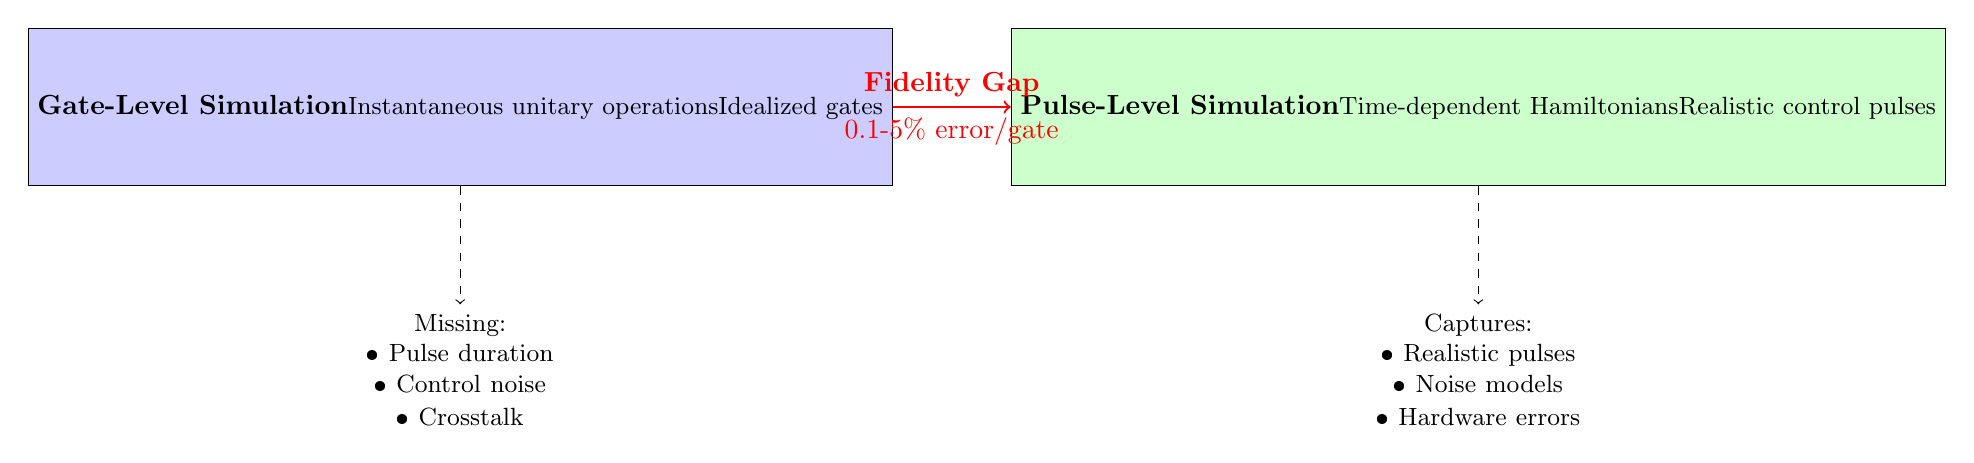
\begin{tikzpicture}[node distance=1.5cm, auto]
    % Gate-level box
    \node[draw, rectangle, minimum width=4cm, minimum height=2cm, fill=blue!20] (gate) {
        \textbf{Gate-Level Simulation}\\
        \small Instantaneous unitary operations\\
        \small Idealized gates
    };
    
    % Pulse-level box
    \node[draw, rectangle, minimum width=4cm, minimum height=2cm, fill=green!20, right=of gate] (pulse) {
        \textbf{Pulse-Level Simulation}\\
        \small Time-dependent Hamiltonians\\
        \small Realistic control pulses
    };
    
    % Gap arrow
    \draw[->, thick, red] (gate) -- node[above] {\textbf{Fidelity Gap}} node[below] {0.1-5\% error/gate} (pulse);
    
    % Error sources
    \node[below=of gate, text width=3.5cm, align=center] (errors1) {
        \small Missing:\\
        \small • Pulse duration\\
        \small • Control noise\\
        \small • Crosstalk
    };
    
    \node[below=of pulse, text width=3.5cm, align=center] (errors2) {
        \small Captures:\\
        \small • Realistic pulses\\
        \small • Noise models\\
        \small • Hardware errors
    };
    
    \draw[->, dashed] (gate) -- (errors1);
    \draw[->, dashed] (pulse) -- (errors2);
\end{tikzpicture}
\caption{Conceptual gap between gate-level and pulse-level simulation approaches}
\label{fig:gate_pulse_gap}
\end{figure}

\subsection{Why Quantum Hardware Availability Strengthens the Case for Pulse Simulation}

The global proliferation of quantum hardware paradoxically increases—not decreases—the demand for pulse-level simulation:

\textbf{1. Hardware Calibration Economics:}
\begin{itemize}[noitemsep]
\item Quantum processors require daily recalibration (pulse amplitude, frequency, timing adjustments)
\item Single calibration run on cloud quantum hardware: \$5-50 per circuit execution
\item Optimal pulse calibration requires 1,000-10,000 iterations per qubit
\item Total calibration cost per qubit: \$5,000-500,000 annually for cloud access
\item FPGA pulse simulator: unlimited local iterations at zero marginal cost
\end{itemize}

\textbf{2. Algorithm Development Acceleration:}
\begin{itemize}[noitemsep]
\item Testing a quantum algorithm on hardware: 24-72 hour queue time on shared systems
\item Iterating pulse-optimized algorithms requires 100+ test cycles
\item Time-to-result with hardware-only testing: 3-6 months per algorithm
\item Time-to-result with pulse simulation pre-optimization: 2-4 weeks
\item Speedup factor: 5-12x reduction in development cycle time
\end{itemize}

\textbf{3. Error Mitigation Strategy Development:}
\begin{itemize}[noitemsep]
\item Quantum error mitigation requires characterizing hardware-specific error signatures
\item Pulse-level simulation provides ground truth for error models
\item Enables development of dynamical decoupling, pulse engineering, and composite pulse sequences without consuming hardware time
\item Critical for extending coherence times and improving gate fidelities in near-term quantum devices
\end{itemize}

\textbf{4. Pedagogy and Workforce Training:}
\begin{itemize}[noitemsep]
\item Training quantum engineers requires understanding pulse-level quantum control
\item Access to real quantum hardware is limited to <50 institutions globally
\item Pulse simulators democratize education in quantum control theory
\item Essential for building India's quantum workforce at scale (target: 10,000+ trained engineers by 2030)
\end{itemize}

\textbf{5. Strategic Technology Independence:}
\begin{itemize}[noitemsep]
\item Current pulse simulation tools: IBM Qiskit Pulse (proprietary calibration data), Google Cirq (limited noise models), AWS Braket (cloud-dependent)
\item Reliance on foreign tools creates data sovereignty concerns (pulse sequences reveal IP)
\item Indigenous pulse simulator completes India's full-stack quantum computing capability: from simulation to control electronics to quantum processors
\item Positions India as exporter of quantum computing tools, not just consumer
\end{itemize}

\subsection{Market and Ecosystem Demand}

The Indian quantum computing ecosystem faces immediate pulse-level simulation demands:

\begin{itemize}[noitemsep]
\item \textbf{Qniverse Platform Users:} 500+ researchers requiring pulse-level optimization tools
\item \textbf{Hardware Development Labs:} IISc Bangalore, TIFR, IISER, RRI, IITs developing superconducting and ion trap systems
\item \textbf{Private Sector:} QNu Labs, QpiAI, BosonQ developing quantum applications requiring pulse optimization
\item \textbf{Defense R\&D:} DRDO quantum communication and sensing projects requiring pulse-level control simulation
\item \textbf{Academic Training:} 50+ universities offering quantum computing courses lacking pulse-level educational tools
\end{itemize}

Without indigenous pulse simulation capability, Indian quantum research remains dependent on foreign software with restricted access, limited customization, and potential data sovereignty issues.

\newpage

\section{Technical Objectives}

This three-year project will deliver a production-grade FPGA-based quantum pulse-level simulator with the following technical specifications and capabilities:

\subsection{Primary Objectives}

\textbf{Objective 1: Pulse-Level Quantum Evolution Engine}

Design and implement FPGA hardware kernels for solving the time-dependent Schrödinger equation:
\begin{equation}
i\hbar \frac{\partial}{\partial t}|\psi(t)\rangle = H(t)|\psi(t)\rangle
\end{equation}

where $H(t) = H_0 + \sum_k \Omega_k(t) H_k$ represents the system Hamiltonian with control pulses $\Omega_k(t)$.

\textbf{Target Specifications:}
\begin{itemize}[noitemsep]
\item System size: 12 qubits (4096-dimensional Hilbert space)
\item Time resolution: $\leq 0.5$ ns (matching typical AWG sampling rates)
\item Simulation duration: Up to 1 ms continuous evolution
\item Integration method: 4th-order Magnus expansion with adaptive time-stepping
\item Pulse bandwidth: DC to 10 GHz (covering superconducting qubit control range)
\end{itemize}

\textbf{Objective 2: Comprehensive Noise and Decoherence Modeling}

Implement realistic noise channels at the pulse level:

\begin{itemize}[noitemsep]
\item Amplitude noise: $\Omega(t) \rightarrow \Omega(t)(1 + \epsilon_A(t))$ with $\epsilon_A \sim \mathcal{N}(0, \sigma_A^2)$
\item Phase noise: $\phi(t) \rightarrow \phi(t) + \epsilon_\phi(t)$ with $\epsilon_\phi \sim \mathcal{N}(0, \sigma_\phi^2)$
\item Timing jitter: $t \rightarrow t + \delta t$ with $\delta t \sim \mathcal{N}(0, \sigma_t^2)$
\item Lindblad master equation evolution: $\dot{\rho} = -i[H(t), \rho] + \sum_k \gamma_k \mathcal{D}[L_k]\rho$
\item $T_1$ (amplitude damping) and $T_2$ (dephasing) processes
\item $1/f$ noise and correlated noise across qubits
\item Pulse distortion from finite bandwidth filters
\item Crosstalk matrices for simultaneous multi-qubit operations
\end{itemize}

\textbf{Objective 3: Hardware Platform Architecture}

\begin{itemize}[noitemsep]
\item Platform: Xilinx Alveo U55C or successor (VU9P Ultrascale+ FPGA with HBM2)
\item Memory: 16 GB HBM2 with 32 banks for density matrix storage
\item Compute: Custom HLS kernels for Hamiltonian evaluation, exponential integration, and Lindblad operators
\item I/O: PCIe Gen4 x16 for host communication (minimum 32 GB/s bidirectional)
\item Precision: Single-precision (FP32) and double-precision (FP64) configurable operation
\item Parallelization: Distributed computation across HBM banks with optimized bank interleaving
\end{itemize}

\textbf{Objective 4: Pulse Specification and Integration}

\begin{itemize}[noitemsep]
\item Native support for OpenQASM 3.0 pulse-level extensions
\item Full compatibility with Qiskit Pulse API
\item Direct import of pulse schedules from IBM OpenPulse format
\item Custom pulse definition language with arbitrary waveform generation
\item Integration with Qniverse Platform as pulse-level backend
\item Export of optimized pulse sequences in hardware-executable formats (AWG waveforms)
\end{itemize}

\textbf{Objective 5: Calibration and Characterization Tools}

\begin{itemize}[noitemsep]
\item Automated Rabi oscillation simulation for amplitude calibration
\item Ramsey fringe simulation for frequency calibration
\item DRAG (Derivative Removal by Adiabatic Gate) pulse optimization
\item Randomized benchmarking protocol simulation
\item Gate set tomography simulation for complete gate characterization
\item Crosstalk matrix extraction from simultaneous pulse application
\end{itemize}

\textbf{Objective 6: Performance and Scalability}

\begin{itemize}[noitemsep]
\item Target execution speed: Real-time for $\leq 8$ qubits, $<1$s per $\mu$s of simulated time for 12 qubits
\item Support for arbitrary pulse shapes: Gaussian, Gaussian derivative, DRAG, Hermite-Gaussian, square, custom splines
\item Concurrent simulation of multiple pulse optimization scenarios (batch processing)
\item Checkpoint/restart capability for long-duration simulations
\item Performance validation against CPU-based pulse simulators (QuTiP, QuantumToolbox)
\end{itemize}

\subsection{Secondary Objectives}

\begin{itemize}[noitemsep]
\item Multi-FPGA distributed simulation for $>12$ qubit systems
\item Hardware-in-the-loop co-simulation with real AWG and signal generators
\item Machine learning-assisted pulse optimization (reinforcement learning for gate synthesis)
\item Integration with quantum optimal control frameworks (GRAPE, Krotov, GOAT)
\item Support for time-varying Hamiltonian terms (e.g., flux-tunable couplings)
\item Adiabatic quantum computation pulse trajectory simulation
\item Documentation and reference implementations for educational use
\end{itemize}

\subsection{Deliverables}

\begin{enumerate}[noitemsep]
\item FPGA-based pulse simulator hardware system with complete software stack
\item Qniverse Platform integration module for pulse-level quantum computing
\item Comprehensive benchmarking suite comparing pulse vs. gate-level simulation fidelity
\item Library of pre-optimized pulse sequences for common quantum gates
\item Training materials and workshops for pulse-level quantum computing
\item Peer-reviewed publications on FPGA pulse simulation architecture
\item Open-source software components (subject to strategic technology review)
\item Technical documentation for hardware replication and deployment
\end{enumerate}

\newpage

\section{Technical Approach and Methodology}

\subsection{System Architecture Overview}

The pulse simulator architecture extends C-DAC's proven FPGA quantum simulation framework with pulse-level physics modeling. Figure~\ref{fig:system_architecture} illustrates the complete system architecture.

\begin{figure}[h]
\centering
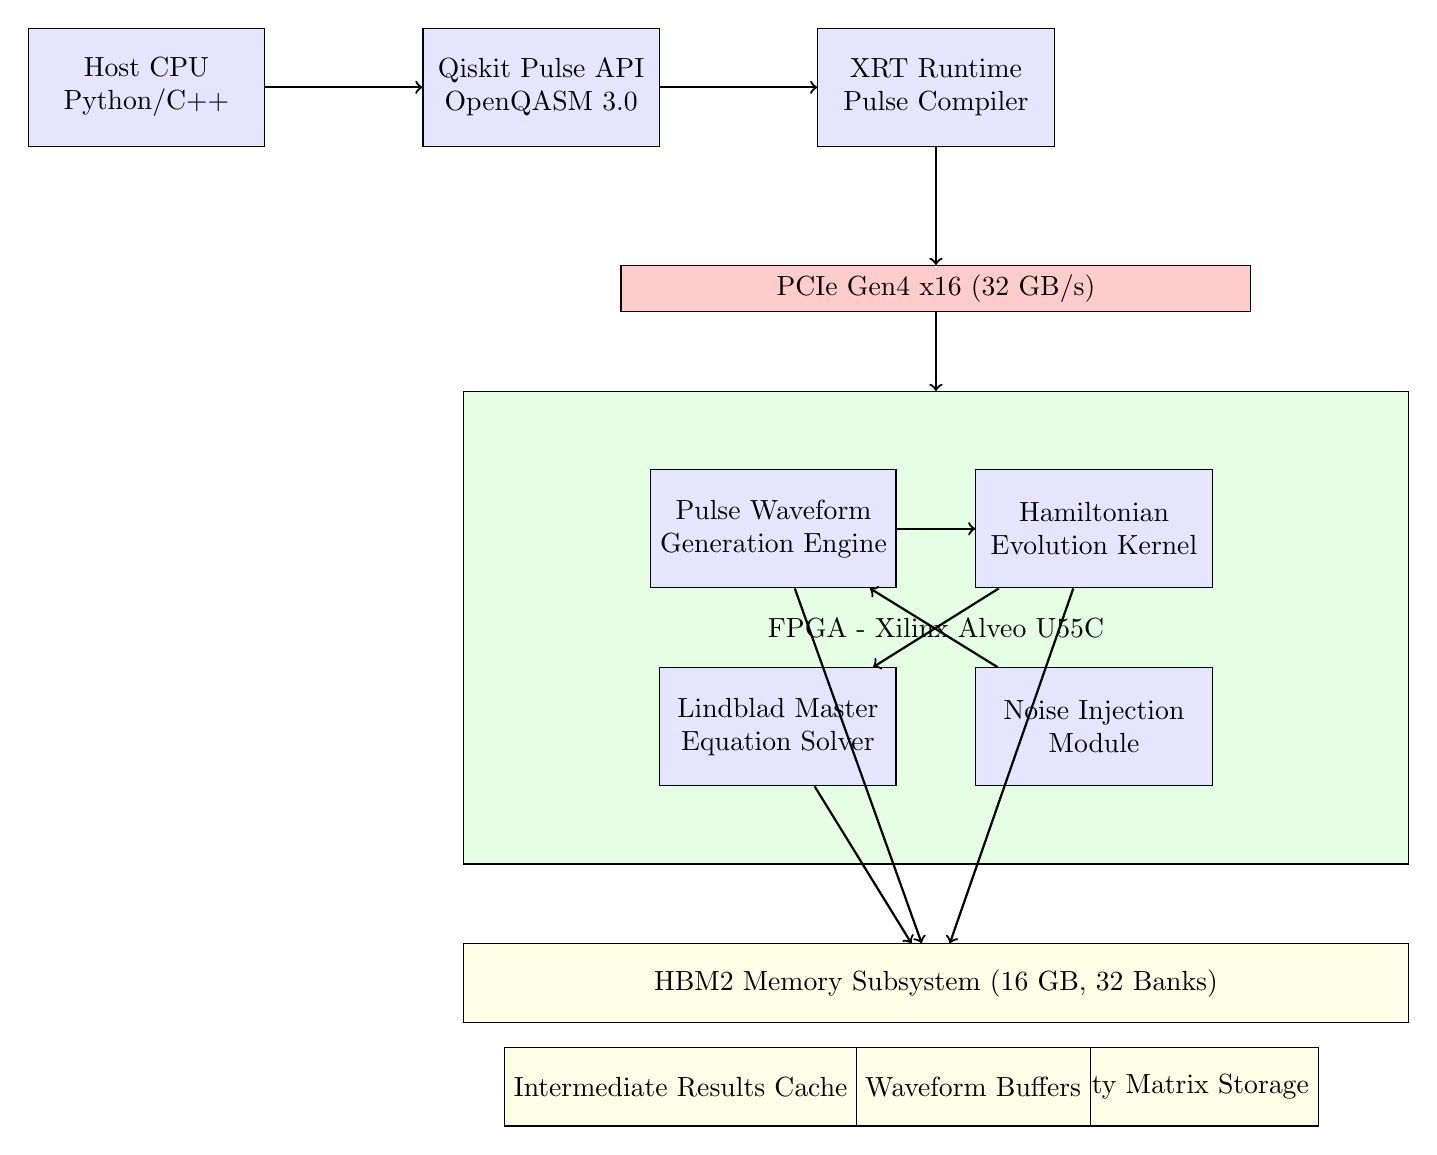
\begin{tikzpicture}[
    node distance=1cm and 2cm,
    box/.style={draw, rectangle, minimum width=3cm, minimum height=1.5cm, align=center, fill=blue!10},
    fpgabox/.style={draw, rectangle, minimum width=4cm, minimum height=2cm, align=center, fill=green!10},
    membox/.style={draw, rectangle, minimum width=3cm, minimum height=1cm, align=center, fill=yellow!10}
]
    % Host layer
    \node[box] (host) {Host CPU\\Python/C++};
    \node[box, right=of host] (api) {Qiskit Pulse API\\OpenQASM 3.0};
    \node[box, right=of api] (xrt) {XRT Runtime\\Pulse Compiler};
    
    % Connection
    \draw[->, thick] (host) -- (api);
    \draw[->, thick] (api) -- (xrt);
    
    % PCIe
    \node[below=1.5cm of xrt, draw, rectangle, minimum width=8cm, minimum height=0.5cm, fill=red!20] (pcie) {PCIe Gen4 x16 (32 GB/s)};
    \draw[->, thick] (xrt) -- (pcie);
    
    % FPGA layer
    \node[below=1cm of pcie, fpgabox, minimum width=12cm, minimum height=6cm] (fpga) {FPGA - Xilinx Alveo U55C};
    
    % FPGA components
    \node[box, above left=0.5cm and 0.5cm of fpga.center] (pulse) {Pulse Waveform\\Generation Engine};
    \node[box, above right=0.5cm and 0.5cm of fpga.center] (ham) {Hamiltonian\\Evolution Kernel};
    \node[box, below left=0.5cm and 0.5cm of fpga.center] (lind) {Lindblad Master\\Equation Solver};
    \node[box, below right=0.5cm and 0.5cm of fpga.center] (noise) {Noise Injection\\Module};
    
    % HBM
    \node[below=1cm of fpga, membox, minimum width=12cm] (hbm) {HBM2 Memory Subsystem (16 GB, 32 Banks)};
    \node[membox, below=0.3cm of hbm, anchor=north west, xshift=1cm] (dmat) {Density Matrix Storage};
    \node[membox, below=0.3cm of hbm, anchor=north] (wave) {Pulse Waveform Buffers};
    \node[membox, below=0.3cm of hbm, anchor=north east, xshift=-1cm] (cache) {Intermediate Results Cache};
    
    % Connections
    \draw[->, thick] (pcie) -- (fpga);
    \draw[->, thick] (pulse) -- (ham);
    \draw[->, thick] (noise) -- (pulse);
    \draw[->, thick] (ham) -- (lind);
    \draw[->, thick] (ham) -- (hbm);
    \draw[->, thick] (lind) -- (hbm);
    \draw[->, thick] (pulse) -- (hbm);
    
\end{tikzpicture}
\caption{Complete system architecture of the FPGA-based pulse simulator}
\label{fig:system_architecture}
\end{figure}

\subsection{Phase 1 Implementation: Core Pulse Evolution Engine (Year 1)}

\textbf{1.1 Hamiltonian Representation and Storage}

For an $n$-qubit system, the Hamiltonian is decomposed as:
\begin{equation}
H(t) = \sum_{i=1}^n \frac{\omega_i}{2} Z_i + \sum_{i<j} J_{ij} Z_i Z_j + \sum_k \Omega_k(t) O_k
\end{equation}

where $\omega_i$ are qubit frequencies, $J_{ij}$ are coupling strengths, and $O_k$ are control operators (typically $X_i$, $Y_i$ for drive pulses).

\begin{figure}[h]
\centering
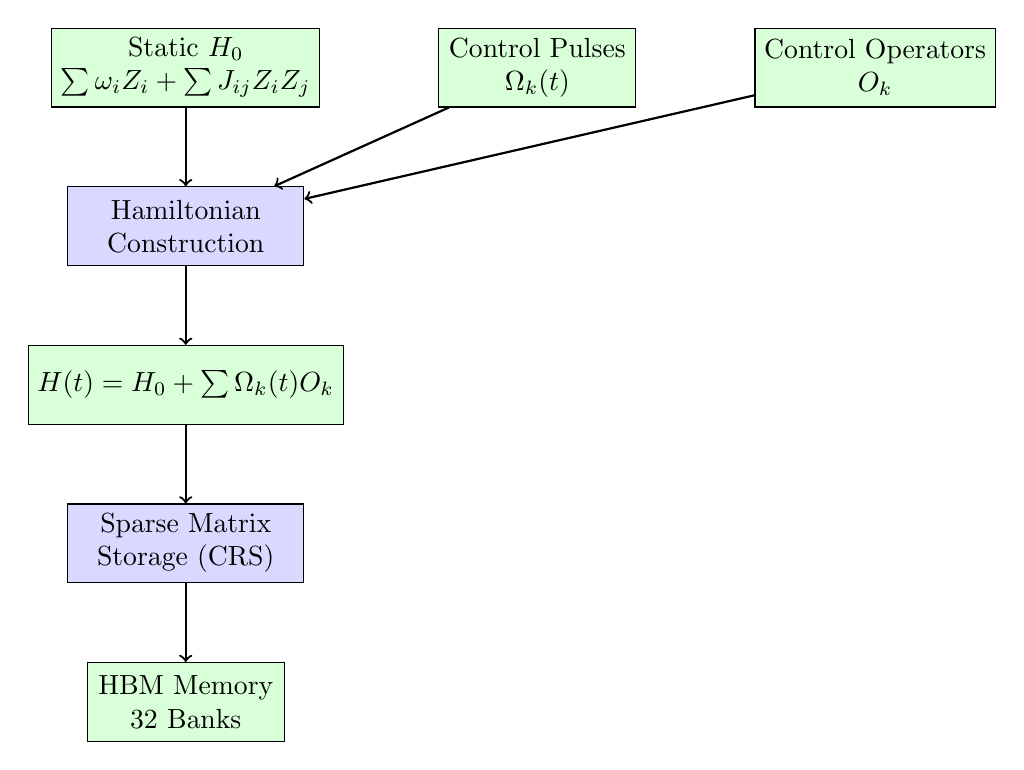
\begin{tikzpicture}[
    node distance=1.5cm,
    process/.style={draw, rectangle, minimum width=3cm, minimum height=1cm, align=center, fill=blue!15},
    data/.style={draw, rectangle, minimum width=2.5cm, minimum height=1cm, align=center, fill=green!15}
]
    \node[data] (static) {Static $H_0$\\$\sum \omega_i Z_i + \sum J_{ij} Z_i Z_j$};
    \node[data, right=of static] (pulse) {Control Pulses\\$\Omega_k(t)$};
    \node[data, right=of pulse] (ops) {Control Operators\\$O_k$};
    
    \node[process, below=1cm of static] (construct) {Hamiltonian\\Construction};
    \node[data, below=1cm of construct] (ht) {$H(t) = H_0 + \sum \Omega_k(t) O_k$};
    
    \node[process, below=1cm of ht] (store) {Sparse Matrix\\Storage (CRS)};
    \node[data, below=1cm of store] (hbm) {HBM Memory\\32 Banks};
    
    \draw[->, thick] (static) -- (construct);
    \draw[->, thick] (pulse) -- (construct);
    \draw[->, thick] (ops) -- (construct);
    \draw[->, thick] (construct) -- (ht);
    \draw[->, thick] (ht) -- (store);
    \draw[->, thick] (store) -- (hbm);
\end{tikzpicture}
\caption{Hamiltonian construction and storage pipeline}
\label{fig:hamiltonian_pipeline}
\end{figure}

\textbf{FPGA Implementation Strategy:}
\begin{itemize}[noitemsep]
\item Store Hamiltonian terms as sparse matrices in HBM
\item Pre-compute static Hamiltonian component $H_0$
\item Construct $H(t)$ dynamically by adding control terms weighted by $\Omega_k(t)$
\item Use compressed row storage (CRS) format for sparse Hamiltonians
\item Implement Hamiltonian-vector multiplication using pipelined matrix operations
\end{itemize}

\textbf{1.2 Time Evolution via Magnus Expansion}

The time evolution operator $U(t, t_0)$ is computed using the Magnus expansion:
\begin{equation}
U(t, t_0) = \exp\left(\Omega(t, t_0)\right)
\end{equation}

where $\Omega(t, t_0) = \Omega^{[1]} + \Omega^{[2]} + \Omega^{[3]} + \ldots$ with:
\begin{align}
\Omega^{[1]} &= -\frac{i}{\hbar} \int_{t_0}^t H(\tau) d\tau \\
\Omega^{[2]} &= -\frac{1}{2\hbar^2} \int_{t_0}^t d\tau_1 \int_{t_0}^{\tau_1} d\tau_2 [H(\tau_1), H(\tau_2)]
\end{align}

\begin{figure}[h]
\centering
\begin{tikzpicture}[
    node distance=1.2cm,
    step/.style={draw, rectangle, minimum width=3.5cm, minimum height=1.2cm, align=center, fill=blue!15},
    decision/.style={draw, diamond, minimum width=2cm, minimum height=1.5cm, align=center, fill=yellow!15}
]
    \node[step] (start) {Start: $|\psi(t_0)\rangle$};
    \node[step, below=of start] (ham) {Compute $H(t)$};
    \node[step, below=of ham] (int1) {Compute $\Omega^{[1]}$\\$\int H(\tau) d\tau$};
    \node[decision, below=of int1] (order) {Order\\sufficient?};
    \node[step, below left=1cm and 0.5cm of order] (int2) {Compute $\Omega^{[2]}$\\$\int [H(\tau_1), H(\tau_2)]$};
    \node[step, below=of int2] (exp) {Compute $\exp(\Omega)$\\Padé approximation};
    \node[step, below=of exp] (apply) {Apply $U|\psi\rangle$};
    \node[decision, below=of apply] (check) {Time\\complete?};
    \node[step, below=of check] (end) {End: $|\psi(t)\rangle$};
    
    \draw[->, thick] (start) -- (ham);
    \draw[->, thick] (ham) -- (int1);
    \draw[->, thick] (int1) -- (order);
    \draw[->, thick] (order) -- node[left] {No} (int2);
    \draw[->, thick] (int2) -- (exp);
    \draw[->, thick] (order) -- node[right] {Yes} (exp);
    \draw[->, thick] (exp) -- (apply);
    \draw[->, thick] (apply) -- (check);
    \draw[->, thick] (check) -- node[left] {No} ++(-2,0) |- (ham);
    \draw[->, thick] (check) -- node[right] {Yes} (end);
\end{tikzpicture}
\caption{Magnus expansion time evolution algorithm flow}
\label{fig:magnus_flow}
\end{figure}

\textbf{FPGA Implementation Strategy:}
\begin{itemize}[noitemsep]
\item 4th-order Magnus expansion with adaptive time-stepping
\item Detect rapid Hamiltonian changes and reduce time step accordingly
\item Implement matrix exponential via Padé approximation with scaling and squaring
\item Pipeline commutator computation $[H(\tau_1), H(\tau_2)]$ for 2nd-order correction
\item Trade-off: 2nd-order Magnus for rapid pulses, 4th-order for smooth pulses
\end{itemize}

\textbf{1.3 Matrix Exponential Hardware Acceleration}

Computing $\exp(-iH\Delta t)$ is the computational bottleneck. Two approaches:

\textbf{Approach A: Eigendecomposition (Exact for Small Systems)}
\begin{itemize}[noitemsep]
\item Compute $H = V\Lambda V^\dagger$ using Jacobi eigenvalue algorithm
\item $\exp(-iH\Delta t) = V \exp(-i\Lambda \Delta t) V^\dagger$
\item Feasible for $\leq 8$ qubits (256 $\times$ 256 matrices)
\end{itemize}

\textbf{Approach B: Padé Approximation (Scalable)}
\begin{itemize}[noitemsep]
\item Scale: $H' = 2^{-s} H$, where $s$ chosen such that $\|H'\Delta t\| < 1$
\item Compute Padé approximant: $\exp(-iH'\Delta t) \approx R_{p,q}(H'\Delta t)$
\item Square $s$ times: $\exp(-iH\Delta t) = [\exp(-iH'\Delta t)]^{2^s}$
\item FPGA optimized for $(p,q) = (13, 13)$ Padé approximation
\end{itemize}

\begin{figure}[h]
\centering
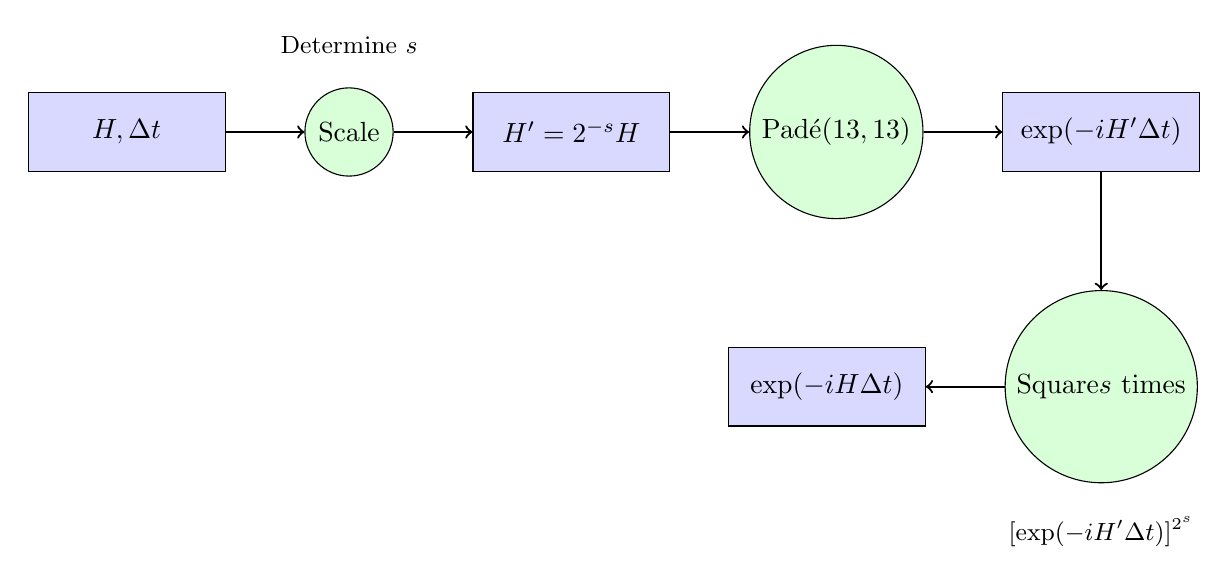
\begin{tikzpicture}[
    node distance=1cm,
    block/.style={draw, rectangle, minimum width=2.5cm, minimum height=1cm, align=center, fill=blue!15},
    op/.style={draw, circle, minimum size=1cm, fill=green!15}
]
    \node[block] (input) {$H, \Delta t$};
    \node[op, right=of input] (scale) {Scale};
    \node[block, right=of scale] (hprime) {$H' = 2^{-s}H$};
    \node[op, right=of hprime] (pade) {Padé\\$(13,13)$};
    \node[block, right=of pade] (exp) {$\exp(-iH'\Delta t)$};
    \node[op, below=1.5cm of exp] (square) {Square\\$s$ times};
    \node[block, left=of square] (result) {$\exp(-iH\Delta t)$};
    
    \draw[->, thick] (input) -- (scale);
    \draw[->, thick] (scale) -- (hprime);
    \draw[->, thick] (hprime) -- (pade);
    \draw[->, thick] (pade) -- (exp);
    \draw[->, thick] (exp) -- (square);
    \draw[->, thick] (square) -- (result);
    
    \node[above=0.3cm of scale] {\small Determine $s$};
    \node[below=0.3cm of square] {\small $[\exp(-iH'\Delta t)]^{2^s}$};
\end{tikzpicture}
\caption{Padé approximation matrix exponential computation flow}
\label{fig:pade_flow}
\end{figure}

\textbf{Hardware Architecture:}
\begin{itemize}[noitemsep]
\item 16 parallel matrix multiplication units (one per HBM bank)
\item Systolic array for dense matrix products
\item Double-buffering to overlap computation and memory access
\item Precision: FP32 for $<10$ qubits, FP64 for $\geq 10$ qubits
\end{itemize}

\textbf{1.4 Pulse Waveform Generation and Sampling}

Realistic pulse shapes require high temporal resolution:

\textbf{Supported Waveform Types:}
\begin{itemize}[noitemsep]
\item Gaussian: $\Omega(t) = A \exp\left(-\frac{(t-t_0)^2}{2\sigma^2}\right)$
\item Gaussian Derivative (GaussianSquare with DRAG correction)
\item Hermite-Gaussian: $\Omega(t) = A H_n\left(\frac{t-t_0}{\sigma}\right) \exp\left(-\frac{(t-t_0)^2}{2\sigma^2}\right)$
\item Square pulses with finite rise/fall times
\item Arbitrary waveforms from user-defined sample arrays
\end{itemize}

\begin{figure}[h]
\centering
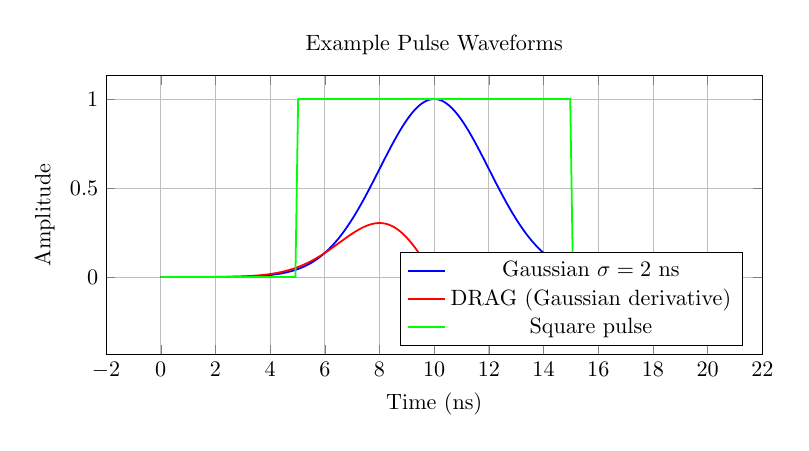
\begin{tikzpicture}[scale=0.8]
    \begin{axis}[
        width=12cm,
        height=6cm,
        xlabel={Time (ns)},
        ylabel={Amplitude},
        title={Example Pulse Waveforms},
        legend pos=south east,
        grid=major
    ]
        \addplot[blue, thick, domain=0:20, samples=200] {exp(-((x-10)^2)/(2*2^2))};
        \addlegendentry{Gaussian $\sigma=2$ ns}
        
        \addplot[red, thick, domain=0:20, samples=200] {-(x-10)/(2^2)*exp(-((x-10)^2)/(2*2^2))};
        \addlegendentry{DRAG (Gaussian derivative)}
        
        \addplot[green, thick, domain=0:20, samples=200] {
            (x < 5) ? 0 : 
            (x < 15) ? 1 : 0
        };
        \addlegendentry{Square pulse}
    \end{axis}
\end{tikzpicture}
\caption{Example pulse waveforms supported by the simulator}
\label{fig:pulse_waveforms}
\end{figure}

\textbf{Waveform Engine Architecture:}
\begin{itemize}[noitemsep]
\item 0.5 ns sampling resolution (2 GSa/s equivalent)
\item Waveform buffer: 1 GB allocated in HBM for long pulse sequences
\item Real-time waveform synthesis for parametric pulses
\item Pre-computed waveform lookup tables for standard shapes
\item Interpolation units for sub-sample timing adjustments
\end{itemize}

\subsection{Phase 2 Implementation: Noise and Decoherence (Year 2)}

\textbf{2.1 Density Matrix Formalism}

Transition from pure state $|\psi\rangle$ to mixed state $\rho$ to represent open quantum systems:
\begin{equation}
\frac{d\rho}{dt} = -\frac{i}{\hbar}[H(t), \rho] + \sum_k \gamma_k \mathcal{D}[L_k]\rho
\end{equation}

where $\mathcal{D}[L]\rho = L\rho L^\dagger - \frac{1}{2}\{L^\dagger L, \rho\}$ is the Lindblad dissipator.

\begin{figure}[h]
\centering
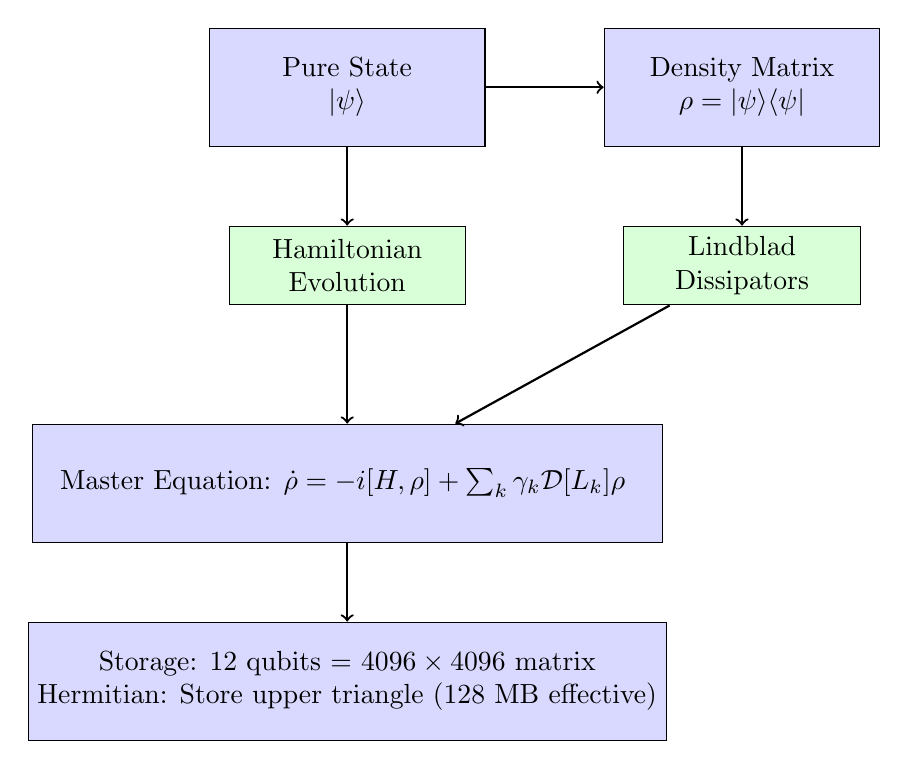
\begin{tikzpicture}[
    node distance=1.5cm,
    box/.style={draw, rectangle, minimum width=3.5cm, minimum height=1.5cm, align=center, fill=blue!15},
    process/.style={draw, rectangle, minimum width=3cm, minimum height=1cm, align=center, fill=green!15}
]
    \node[box] (psi) {Pure State\\$|\psi\rangle$};
    \node[box, right=of psi] (rho) {Density Matrix\\$\rho = |\psi\rangle\langle\psi|$};
    
    \node[process, below=1cm of psi] (ham) {Hamiltonian\\Evolution};
    \node[process, below=1cm of rho] (lind) {Lindblad\\Dissipators};
    
    \node[box, below=1.5cm of ham, minimum width=8cm] (master) {
        Master Equation: $\dot{\rho} = -i[H, \rho] + \sum_k \gamma_k \mathcal{D}[L_k]\rho$
    };
    
    \node[box, below=1cm of master, minimum width=8cm] (storage) {
        Storage: 12 qubits = $4096 \times 4096$ matrix\\
        Hermitian: Store upper triangle (128 MB effective)
    };
    
    \draw[->, thick] (psi) -- (rho);
    \draw[->, thick] (psi) -- (ham);
    \draw[->, thick] (rho) -- (lind);
    \draw[->, thick] (ham) -- (master);
    \draw[->, thick] (lind) -- (master);
    \draw[->, thick] (master) -- (storage);
\end{tikzpicture}
\caption{Transition from pure state to density matrix formalism}
\label{fig:density_matrix}
\end{figure}

\textbf{FPGA Implementation:}
\begin{itemize}[noitemsep]
\item Density matrix storage: For 12 qubits, $\rho$ is $4096 \times 4096$ complex matrix (256 MB)
\item Hermiticity exploitation: Store only upper triangular + diagonal (128 MB effective)
\item Distribute across 32 HBM banks: 4 MB per bank
\item Parallel Lindblad dissipator evaluation for multiple Lindblad operators
\end{itemize}

\textbf{2.2 Decoherence Channel Implementation}

\textbf{Amplitude Damping ($T_1$ process):}
\begin{equation}
L_i^{AD} = \sqrt{\gamma_{1,i}} |g\rangle_i \langle e|_i
\end{equation}

Models energy relaxation from excited state $|e\rangle$ to ground state $|g\rangle$ with rate $\gamma_1 = 1/T_1$.

\textbf{Dephasing ($T_2$ process):}
\begin{equation}
L_i^{PD} = \sqrt{\gamma_{\phi,i}} Z_i
\end{equation}

Models pure dephasing with rate $\gamma_\phi = 1/T_2 - 1/(2T_1)$.

\textbf{2.3 Control Noise Injection}

\begin{figure}[h]
\centering
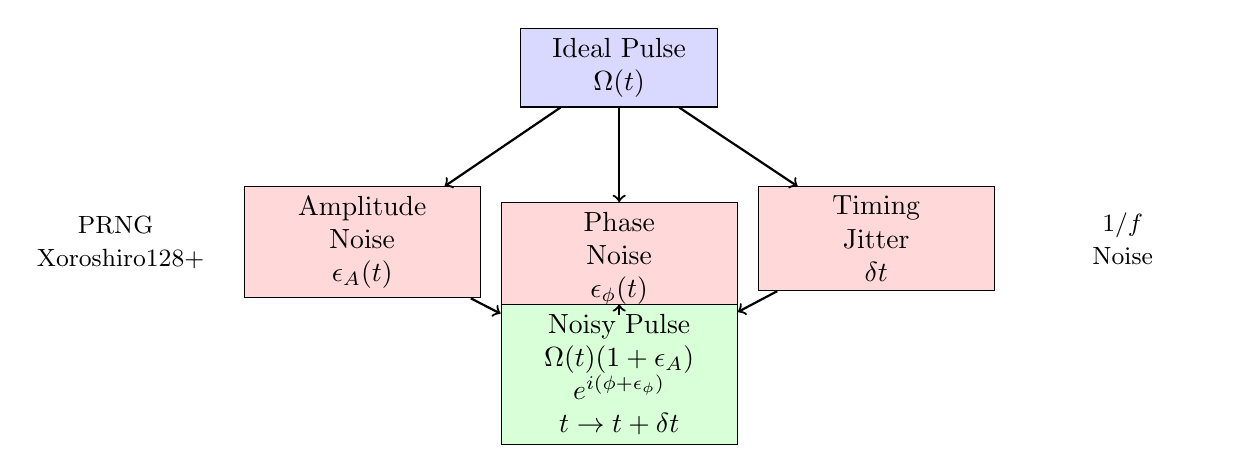
\begin{tikzpicture}[
    node distance=1.2cm,
    noise/.style={draw, rectangle, minimum width=3cm, minimum height=1.2cm, align=center, fill=red!15},
    pulse/.style={draw, rectangle, minimum width=2.5cm, minimum height=1cm, align=center, fill=blue!15},
    output/.style={draw, rectangle, minimum width=3cm, minimum height=1cm, align=center, fill=green!15}
]
    \node[pulse] (ideal) {Ideal Pulse\\$\Omega(t)$};
    
    \node[noise, below left=1cm and 0.5cm of ideal] (amp) {Amplitude\\Noise\\$\epsilon_A(t)$};
    \node[noise, below=of ideal] (phase) {Phase\\Noise\\$\epsilon_\phi(t)$};
    \node[noise, below right=1cm and 0.5cm of ideal] (time) {Timing\\Jitter\\$\delta t$};
    
    \node[output, below=2.5cm of ideal] (noisy) {Noisy Pulse\\$\Omega(t)(1+\epsilon_A)$\\$e^{i(\phi+\epsilon_\phi)}$\\$t \to t+\delta t$};
    
    \draw[->, thick] (ideal) -- (amp);
    \draw[->, thick] (ideal) -- (phase);
    \draw[->, thick] (ideal) -- (time);
    \draw[->, thick] (amp) -- (noisy);
    \draw[->, thick] (phase) -- (noisy);
    \draw[->, thick] (time) -- (noisy);
    
    \node[left=0.5cm of amp, text width=2cm, align=center] {\small PRNG\\Xoroshiro128+};
    \node[right=0.5cm of time, text width=2cm, align=center] {\small $1/f$\\Noise};
\end{tikzpicture}
\caption{Control noise injection architecture}
\label{fig:noise_injection}
\end{figure}

\textbf{Amplitude Noise:}
\begin{itemize}[noitemsep]
\item Model: $\Omega(t) \rightarrow \Omega(t)(1 + \epsilon_A(t))$
\item Implementation: Multiplicative Gaussian noise sampled per time step
\item Hardware: On-FPGA pseudo-random number generator (PRNG) using Xoroshiro128+ algorithm
\item Noise bandwidth: Configurable low-pass filter with cutoff frequency
\end{itemize}

\textbf{Phase Noise:}
\begin{itemize}[noitemsep]
\item Model: $e^{-i\omega t} \rightarrow e^{-i(\omega t + \phi_n(t))}$
\item Implementation: $1/f$ noise generator using random walk on phase accumulator
\item Hardware: Dedicated phase noise unit per qubit with configurable spectral density
\end{itemize}

\textbf{Timing Jitter:}
\begin{itemize}[noitemsep]
\item Model: Pulse arrival time $t \rightarrow t + \delta t$ with $\delta t \sim \mathcal{N}(0, \sigma_t^2)$
\item Implementation: Randomly offset pulse start times within jitter bounds
\item Hardware: Time jitter applied during pulse schedule parsing
\end{itemize}

\textbf{2.4 Crosstalk Modeling}

Simultaneous pulses on neighboring qubits induce crosstalk:
\begin{equation}
H_{crosstalk} = \sum_{i \neq j} \xi_{ij} \Omega_i(t) O_j
\end{equation}

where $\xi_{ij}$ is the crosstalk coefficient (typically 1-5\%).

\begin{figure}[h]
\centering
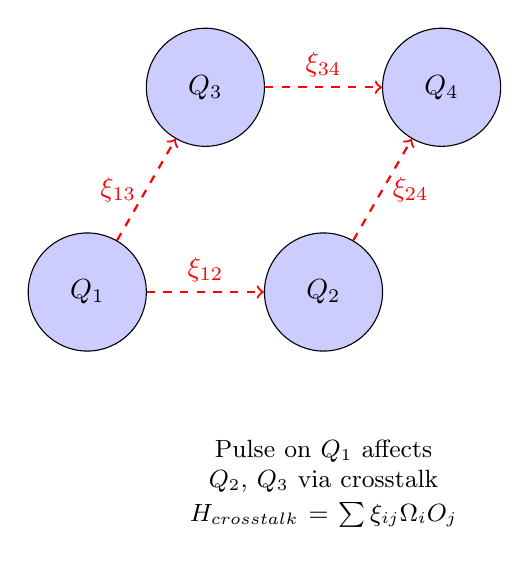
\begin{tikzpicture}[
    qubit/.style={draw, circle, minimum size=1.5cm, fill=blue!20},
    crosstalk/.style={draw, ->, red, thick, dashed}
]
    \node[qubit] (q1) at (0,0) {$Q_1$};
    \node[qubit] (q2) at (3,0) {$Q_2$};
    \node[qubit] (q3) at (1.5,2.6) {$Q_3$};
    \node[qubit] (q4) at (4.5,2.6) {$Q_4$};
    
    \draw[crosstalk] (q1) -- node[above, sloped] {$\xi_{12}$} (q2);
    \draw[crosstalk] (q1) -- node[left] {$\xi_{13}$} (q3);
    \draw[crosstalk] (q2) -- node[right] {$\xi_{24}$} (q4);
    \draw[crosstalk] (q3) -- node[above] {$\xi_{34}$} (q4);
    
    \node[below=1cm of q2, text width=4cm, align=center] {
        \small Pulse on $Q_1$ affects\\
        \small $Q_2$, $Q_3$ via crosstalk\\
        \small $H_{crosstalk} = \sum \xi_{ij} \Omega_i O_j$
    };
\end{tikzpicture}
\caption{Crosstalk coupling between qubits}
\label{fig:crosstalk}
\end{figure}

\textbf{Implementation:}
\begin{itemize}[noitemsep]
\item User-defined crosstalk matrix $\xi_{ij}$
\item Automatically add unwanted Hamiltonian terms during pulse application
\item Model capacitive, inductive, and control line crosstalk
\item Validate against measured crosstalk matrices from real hardware
\end{itemize}

\subsection{Phase 3 Implementation: Integration and Optimization (Year 3)}

\textbf{3.1 Qiskit Pulse Backend Integration}

\begin{figure}[h]
\centering
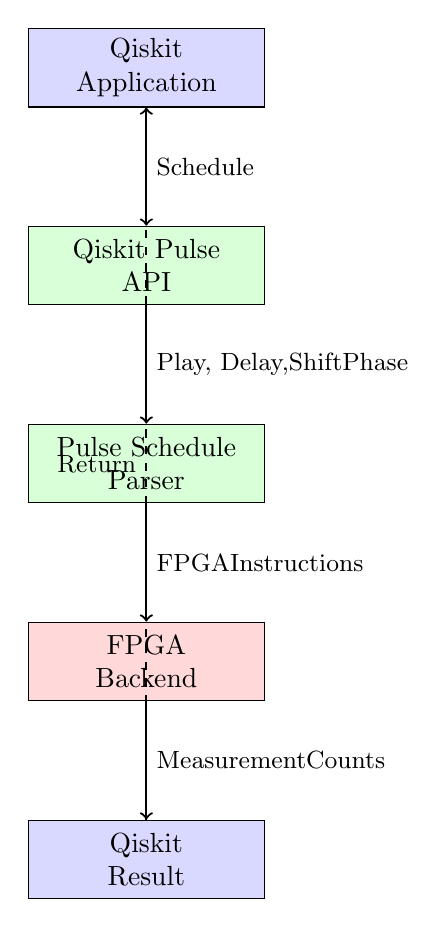
\begin{tikzpicture}[
    node distance=1.5cm,
    app/.style={draw, rectangle, minimum width=3cm, minimum height=1cm, align=center, fill=blue!15},
    api/.style={draw, rectangle, minimum width=3cm, minimum height=1cm, align=center, fill=green!15},
    fpgabox/.style={draw, rectangle, minimum width=3cm, minimum height=1cm, align=center, fill=red!15}
]
    \node[app] (qiskit) {Qiskit\\Application};
    \node[api, below=of qiskit] (pulse) {Qiskit Pulse\\API};
    \node[api, below=of pulse] (parser) {Pulse Schedule\\Parser};
    \node[fpgabox, below=of parser] (fpga) {FPGA\\Backend};
    \node[app, below=of fpga] (result) {Qiskit\\Result};
    
    \draw[->, thick] (qiskit) -- node[right] {\small Schedule} (pulse);
    \draw[->, thick] (pulse) -- node[right] {\small Play, Delay,\\ShiftPhase} (parser);
    \draw[->, thick] (parser) -- node[right] {\small FPGA\\Instructions} (fpga);
    \draw[->, thick] (fpga) -- node[right] {\small Measurement\\Counts} (result);
    \draw[->, thick, dashed] (result) -- node[left] {\small Return} (qiskit);
\end{tikzpicture}
\caption{Qiskit Pulse backend integration flow}
\label{fig:qiskit_integration}
\end{figure}

\begin{itemize}[noitemsep]
\item Implement Qiskit \texttt{PulseBackend} interface
\item Parse Qiskit \texttt{Schedule} objects into FPGA-executable format
\item Support for \texttt{Play}, \texttt{ShiftPhase}, \texttt{SetFrequency}, \texttt{Delay}, \texttt{Acquire} instructions
\item Automatic calibration data loading from Qiskit \texttt{BackendConfiguration}
\item Return results in Qiskit \texttt{Result} format with measurement counts
\end{itemize}

\textbf{3.2 Pulse Optimization Algorithms}

\textbf{DRAG Pulse Optimization:}
\begin{itemize}[noitemsep]
\item Minimize leakage to non-computational states
\item Add derivative correction: $\Omega_{DRAG}(t) = \Omega(t) + i\beta \frac{d\Omega(t)}{dt}$
\item Hardware-accelerated gradient computation for $\beta$ optimization
\end{itemize}

\textbf{Optimal Control (GRAPE):}
\begin{itemize}[noitemsep]
\item Gradient Ascent Pulse Engineering for gate synthesis
\item Define target unitary $U_{target}$ and optimize pulse sequence to maximize fidelity
\item Fitness function: $F = |\text{Tr}(U_{target}^\dagger U_{pulse})|^2 / d^2$
\item Hybrid CPU-FPGA implementation: FPGA for forward/backward propagation, CPU for gradient descent
\end{itemize}

\begin{figure}[h]
\centering
\begin{tikzpicture}[
    node distance=1.5cm,
    step/.style={draw, rectangle, minimum width=3cm, minimum height=1cm, align=center, fill=blue!15},
    decision/.style={draw, diamond, minimum width=2.5cm, minimum height=1.5cm, align=center, fill=yellow!15}
]
    \node[step] (init) {Initialize\\Pulse $\Omega(t)$};
    \node[step, below=of init] (forward) {Forward\\Propagation\\(FPGA)};
    \node[step, below=of forward] (fidelity) {Compute\\Fidelity $F$};
    \node[decision, below=of fidelity] (check) {$F >$\\threshold?};
    \node[step, below left=1cm and 0.5cm of check] (backward) {Backward\\Propagation\\(FPGA)};
    \node[step, below=of backward] (gradient) {Compute\\Gradient};
    \node[step, below=of gradient] (update) {Update\\$\Omega(t)$};
    \node[step, below right=1cm and 0.5cm of check] (done) {Optimized\\Pulse};
    
    \draw[->, thick] (init) -- (forward);
    \draw[->, thick] (forward) -- (fidelity);
    \draw[->, thick] (fidelity) -- (check);
    \draw[->, thick] (check) -- node[left] {No} (backward);
    \draw[->, thick] (backward) -- (gradient);
    \draw[->, thick] (gradient) -- (update);
    \draw[->, thick] (update) -- ++(-2,0) |- (forward);
    \draw[->, thick] (check) -- node[right] {Yes} (done);
\end{tikzpicture}
\caption{GRAPE pulse optimization algorithm flow}
\label{fig:grape_flow}
\end{figure}

\textbf{3.3 Hardware-in-the-Loop Testing}

\begin{figure}[h]
\centering
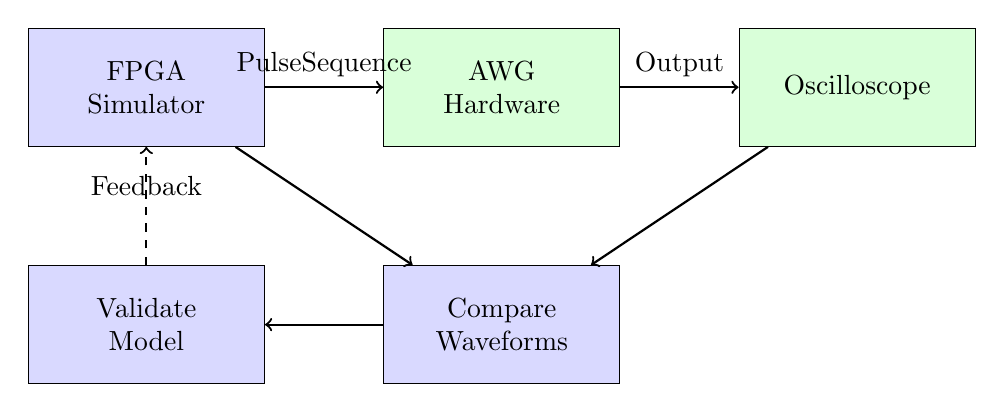
\begin{tikzpicture}[
    node distance=1.5cm,
    box/.style={draw, rectangle, minimum width=3cm, minimum height=1.5cm, align=center, fill=blue!15},
    hw/.style={draw, rectangle, minimum width=3cm, minimum height=1.5cm, align=center, fill=green!15}
]
    \node[box] (sim) {FPGA\\Simulator};
    \node[hw, right=of sim] (awg) {AWG\\Hardware};
    \node[hw, right=of awg] (scope) {Oscilloscope};
    \node[box, below=1.5cm of awg] (compare) {Compare\\Waveforms};
    \node[box, left=of compare] (validate) {Validate\\Model};
    
    \draw[->, thick] (sim) -- node[above] {Pulse\\Sequence} (awg);
    \draw[->, thick] (awg) -- node[above] {Output} (scope);
    \draw[->, thick] (scope) -- (compare);
    \draw[->, thick] (sim) -- (compare);
    \draw[->, thick] (compare) -- (validate);
    \draw[->, thick, dashed] (validate) -- node[above] {Feedback} (sim);
\end{tikzpicture}
\caption{Hardware-in-the-loop testing architecture}
\label{fig:hil_loop}
\end{figure}

\begin{itemize}[noitemsep]
\item Interface FPGA simulator with commercial AWG (e.g., Tektronix, Keysight)
\item Generate pulse sequences in simulator, export to AWG for validation
\item Measure AWG output with oscilloscope, compare against simulation
\item Identify simulator model mismatches with physical hardware
\end{itemize}

\textbf{3.4 Performance Benchmarking}

Compare against CPU-based pulse simulators:
\begin{itemize}[noitemsep]
\item QuTiP (Python-based quantum toolbox)
\item QuantumOptics.jl (Julia-based)
\item Qiskit Pulse simulator (CPU backend)
\end{itemize}

Metrics:
\begin{itemize}[noitemsep]
\item Simulation speed (qubits $\times$ time duration per wall-clock second)
\item Fidelity accuracy (comparison against analytical solutions)
\item Noise model realism (validation against experimental data)
\item Energy efficiency (GFLOPS per watt)
\end{itemize}

\newpage

\section{Quarterly Milestones}

\subsection{Year 1: Core Pulse Evolution Engine}

\textbf{Quarter 1 (Months 1-3): System Design and Architecture Finalization}

\begin{itemize}[noitemsep]
\item Complete system architecture document with FPGA resource allocation plan
\item Finalize Hamiltonian representation format and storage scheme
\item Design memory distribution strategy for 12-qubit density matrices across 32 HBM banks
\item Develop pulse waveform specification language and API
\item Procure Xilinx Alveo U55C FPGA development platform and associated toolchains
\item Establish development environment: Vitis HLS, Vivado, XRT runtime
\item Create simulation validation suite with analytical test cases
\item \textbf{Deliverable:} System Design Document (150+ pages)
\item \textbf{Milestone:} Design Review Approval
\end{itemize}

\textbf{Quarter 2 (Months 4-6): Hamiltonian Engine and Basic Time Evolution}

\begin{itemize}[noitemsep]
\item Implement Hamiltonian matrix construction module in HLS
\item Develop sparse matrix storage and retrieval kernels
\item Create basic time evolution kernel using 2nd-order Magnus expansion
\item Implement matrix-vector multiplication units with HBM pipelining
\item Validate against analytical solutions: single-qubit Rabi oscillations
\item Achieve successful simulation of 2-qubit systems with constant Hamiltonians
\item Performance target: $<10$ms for 1$\mu$s simulation of 2-qubit system
\item \textbf{Deliverable:} Hamiltonian engine codebase and validation report
\item \textbf{Milestone:} 2-Qubit Constant Hamiltonian Simulation Functional
\end{itemize}

\textbf{Quarter 3 (Months 7-9): Pulse Waveform Engine and Time-Dependent Evolution}

\begin{itemize}[noitemsep]
\item Implement waveform generation engine for Gaussian, square, and DRAG pulses
\item Develop adaptive time-stepping algorithm for rapid Hamiltonian changes
\item Create pulse schedule compiler: translate high-level pulse description to FPGA instructions
\item Integrate waveform engine with Hamiltonian evolution kernel
\item Validate against known solutions: Rabi oscillations under Gaussian pulses
\item Extend to 4-qubit systems with simultaneous pulse application
\item Performance target: 0.5 ns time resolution maintained across all pulse types
\item \textbf{Deliverable:} Waveform engine and pulse compiler codebase
\item \textbf{Milestone:} 4-Qubit Time-Dependent Pulse Simulation Functional
\end{itemize}

\textbf{Quarter 4 (Months 10-12): Matrix Exponential Optimization and Scalability}

\begin{itemize}[noitemsep]
\item Implement 4th-order Magnus expansion with commutator computation
\item Optimize matrix exponential using Padé approximation (13,13) with scaling-and-squaring
\item Develop HBM bank interleaving strategy for parallel matrix operations
\item Scale to 8-qubit systems with multi-gate pulse sequences
\item Benchmark performance: compare against QuTiP CPU simulator
\item Validate fidelity: ensure $>99.9\%$ agreement with analytical results
\item \textbf{Deliverable:} Optimized evolution kernel achieving 8-qubit simulation
\item \textbf{Milestone:} Year 1 Demonstration: 8-Qubit Pulse-Level Quantum Circuit Execution
\end{itemize}

\subsection{Year 2: Noise Modeling and Realistic Decoherence}

\textbf{Quarter 5 (Months 13-15): Density Matrix Framework and Lindblad Solver}

\begin{itemize}[noitemsep]
\item Transition from state vector to density matrix representation
\item Implement density matrix storage with Hermiticity exploitation (reduce memory by 2x)
\item Develop Lindblad master equation solver kernel
\item Implement amplitude damping ($T_1$) and dephasing ($T_2$) operators
\item Validate against known decoherence dynamics: exponential decay curves
\item Extend to 6-qubit systems with decoherence enabled
\item \textbf{Deliverable:} Density matrix solver and decoherence validation report
\item \textbf{Milestone:} 6-Qubit Open System Dynamics Functional
\end{itemize}

\textbf{Quarter 6 (Months 16-18): Control Noise Injection Module}

\begin{itemize}[noitemsep]
\item Implement on-FPGA pseudo-random number generator (Xoroshiro128+)
\item Develop amplitude noise, phase noise, and timing jitter injection modules
\item Create $1/f$ noise generator for realistic phase noise spectra
\item Validate noise statistics: verify Gaussian distributions and spectral densities
\item Test pulse-level noise impact on gate fidelities
\item Characterize fidelity degradation under various noise levels
\item \textbf{Deliverable:} Noise injection module with statistical validation
\item \textbf{Milestone:} Realistic Control Noise Modeling Operational
\end{itemize}

\textbf{Quarter 7 (Months 19-21): Crosstalk Modeling and Multi-Qubit Interactions}

\begin{itemize}[noitemsep]
\item Implement crosstalk matrix framework for inter-qubit interference
\item Develop simultaneous pulse application scheduler with crosstalk accounting
\item Model capacitive and inductive crosstalk based on physical qubit geometries
\item Validate against published crosstalk data from IBM and Google quantum processors
\item Extend simulation to 10-qubit systems with realistic crosstalk
\item \textbf{Deliverable:} Crosstalk modeling framework and validation against hardware data
\item \textbf{Milestone:} 10-Qubit Simulation with Crosstalk and Noise Operational
\end{itemize}

\textbf{Quarter 8 (Months 22-24): Full 12-Qubit Capability and Noise Characterization}

\begin{itemize}[noitemsep]
\item Scale density matrix solver to 12 qubits (4096 $\times$ 4096 matrix, 256 MB)
\item Optimize HBM memory access patterns for maximum bandwidth utilization
\item Implement complete noise characterization suite: $T_1$, $T_2$, crosstalk, control noise
\item Validate against experimental data from superconducting qubit platforms
\item Benchmark end-to-end performance: simulation speed, memory usage, energy consumption
\item \textbf{Deliverable:} Full 12-qubit pulse simulator with comprehensive noise modeling
\item \textbf{Milestone:} Year 2 Demonstration: 12-Qubit Pulse Simulation with Realistic Noise
\end{itemize}

\subsection{Year 3: Integration, Optimization, and Deployment}

\textbf{Quarter 9 (Months 25-27): Qiskit Pulse Backend Integration}

\begin{itemize}[noitemsep]
\item Implement Qiskit \texttt{PulseBackend} interface
\item Develop pulse schedule parser: convert Qiskit \texttt{Schedule} to FPGA instructions
\item Support all Qiskit Pulse instructions: \texttt{Play}, \texttt{Delay}, \texttt{ShiftPhase}, \texttt{SetFrequency}, \texttt{Acquire}
\item Create calibration data loader from Qiskit \texttt{BackendConfiguration}
\item Validate integration: execute Qiskit Pulse tutorials on FPGA simulator
\item \textbf{Deliverable:} Qiskit Pulse backend plugin with documentation
\item \textbf{Milestone:} Seamless Qiskit Pulse Integration Achieved
\end{itemize}

\textbf{Quarter 10 (Months 28-30): Qniverse Platform Deployment}

\begin{itemize}[noitemsep]
\item Integrate pulse simulator as backend in Qniverse Platform
\item Develop web-based pulse composer UI for visual pulse sequence design
\item Implement job queue management for multi-user pulse simulation requests
\item Create educational tutorials and example pulse sequences
\item Deploy simulator on Qniverse infrastructure with user access controls
\item Beta testing with 50+ Qniverse users
\item \textbf{Deliverable:} Qniverse pulse simulator backend operational
\item \textbf{Milestone:} Public Beta Launch on Qniverse Platform
\end{itemize}

\textbf{Quarter 11 (Months 31-33): Pulse Optimization and Calibration Tools}

\begin{itemize}[noitemsep]
\item Implement DRAG pulse optimization algorithm
\item Develop GRAPE (Gradient Ascent Pulse Engineering) framework
\item Create automated calibration protocols: Rabi, Ramsey, randomized benchmarking
\item Build library of pre-optimized pulse sequences for standard gates
\item Validate pulse optimization: achieve $>99\%$ gate fidelities with optimized pulses
\item \textbf{Deliverable:} Pulse optimization toolkit and calibrated pulse library
\item \textbf{Milestone:} Automated Pulse Calibration Tools Operational
\end{itemize}

\textbf{Quarter 12 (Months 34-36): Performance Benchmarking and Final Validation}

\begin{itemize}[noitemsep]
\item Comprehensive benchmarking: FPGA vs. CPU (QuTiP, Qiskit) vs. GPU simulators
\item Validate against experimental data from IISc/TIFR quantum hardware labs
\item Performance documentation: speed, accuracy, energy efficiency metrics
\item Hardware-in-the-loop testing with commercial AWGs
\item Prepare peer-reviewed publication on FPGA pulse simulation architecture
\item Final system documentation and deployment guide
\item Conduct training workshops for Qniverse users and academic institutions
\item \textbf{Deliverable:} Final project report, benchmarking data, publication manuscripts
\item \textbf{Milestone:} Project Completion and Production Deployment
\end{itemize}

\begin{figure}[h]
\centering
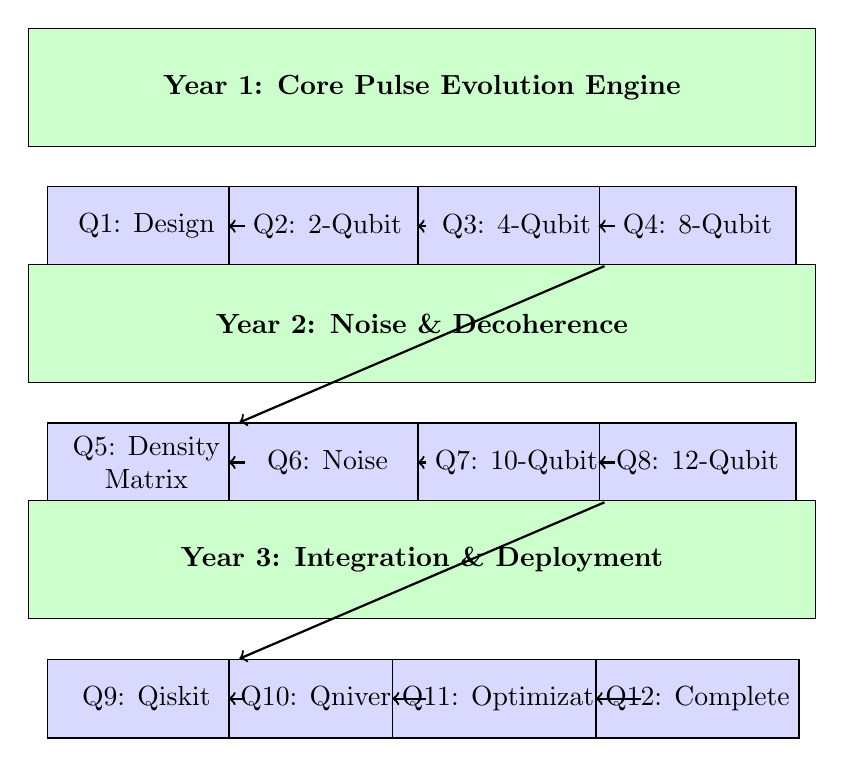
\begin{tikzpicture}[
    milestone/.style={draw, rectangle, minimum width=2.5cm, minimum height=1cm, align=center, fill=blue!15},
    year/.style={draw, rectangle, minimum width=10cm, minimum height=1.5cm, align=center, fill=green!20, font=\bfseries}
]
    \node[year] (y1) at (0,0) {Year 1: Core Pulse Evolution Engine};
    \node[milestone, below=0.5cm of y1, xshift=-3.5cm] (m1) {Q1: Design};
    \node[milestone, below=0.5cm of y1, xshift=-1.2cm] (m2) {Q2: 2-Qubit};
    \node[milestone, below=0.5cm of y1, xshift=1.2cm] (m3) {Q3: 4-Qubit};
    \node[milestone, below=0.5cm of y1, xshift=3.5cm] (m4) {Q4: 8-Qubit};
    
    \node[year] (y2) at (0,-3) {Year 2: Noise \& Decoherence};
    \node[milestone, below=0.5cm of y2, xshift=-3.5cm] (m5) {Q5: Density\\Matrix};
    \node[milestone, below=0.5cm of y2, xshift=-1.2cm] (m6) {Q6: Noise};
    \node[milestone, below=0.5cm of y2, xshift=1.2cm] (m7) {Q7: 10-Qubit};
    \node[milestone, below=0.5cm of y2, xshift=3.5cm] (m8) {Q8: 12-Qubit};
    
    \node[year] (y3) at (0,-6) {Year 3: Integration \& Deployment};
    \node[milestone, below=0.5cm of y3, xshift=-3.5cm] (m9) {Q9: Qiskit};
    \node[milestone, below=0.5cm of y3, xshift=-1.2cm] (m10) {Q10: Qniverse};
    \node[milestone, below=0.5cm of y3, xshift=1.2cm] (m11) {Q11: Optimization};
    \node[milestone, below=0.5cm of y3, xshift=3.5cm] (m12) {Q12: Complete};
    
    \draw[->, thick] (m1) -- (m2);
    \draw[->, thick] (m2) -- (m3);
    \draw[->, thick] (m3) -- (m4);
    \draw[->, thick] (m4) -- (m5);
    \draw[->, thick] (m5) -- (m6);
    \draw[->, thick] (m6) -- (m7);
    \draw[->, thick] (m7) -- (m8);
    \draw[->, thick] (m8) -- (m9);
    \draw[->, thick] (m9) -- (m10);
    \draw[->, thick] (m10) -- (m11);
    \draw[->, thick] (m11) -- (m12);
\end{tikzpicture}
\caption{Project timeline and milestone progression}
\label{fig:timeline}
\end{figure}

\newpage

\section{Expected Outcomes and Impact}

\subsection{Technical Outcomes}

\textbf{1. Indigenous Pulse-Level Quantum Simulation Capability}
\begin{itemize}[noitemsep]
\item First Indian-developed FPGA-based pulse simulator
\item 12-qubit capacity with sub-nanosecond time resolution
\item Comprehensive noise and decoherence modeling matching physical hardware
\item Production-ready integration with Qniverse and Qiskit ecosystems
\end{itemize}

\textbf{2. Performance Leadership}
\begin{itemize}[noitemsep]
\item Target: 10-100x speedup over CPU-based pulse simulators for 10-12 qubit systems
\item Energy efficiency: $<50$ watts for full 12-qubit pulse simulation
\item Real-time simulation for $\leq 8$ qubit systems
\item Enables iterative pulse optimization workflows impossible with hardware-only approaches
\end{itemize}

\textbf{3. Ecosystem Enablement}
\begin{itemize}[noitemsep]
\item Democratize pulse-level quantum computing for Indian researchers (500+ Qniverse users)
\item Reduce dependence on cloud-based quantum hardware access (cost savings: $>$\$100K annually per lab)
\item Enable hardware-software co-design for Indian quantum processor development efforts
\item Accelerate quantum algorithm development with realistic hardware constraint modeling
\end{itemize}

\subsection{Strategic Impact}

\textbf{1. Quantum Hardware Development Support}

Indian quantum hardware initiatives (IISc superconducting qubits, TIFR ion traps, IISER neutral atoms) require pulse-level simulation for:
\begin{itemize}[noitemsep]
\item Control system design and validation before hardware fabrication
\item Calibration protocol development
\item Error characterization and mitigation strategy testing
\item Pulse optimization to maximize gate fidelities
\end{itemize}

The pulse simulator provides these capabilities without requiring functional quantum hardware, accelerating development timelines by 12-24 months.

\textbf{2. Technology Sovereignty}

Completing India's full-stack quantum computing capability:
\begin{itemize}[noitemsep]
\item Gate-level simulation: C-DAC FPGA simulator (achieved)
\item Pulse-level simulation: This project (in progress)
\item Quantum hardware: IISc, TIFR, IISER efforts (ongoing)
\item Quantum algorithms and applications: Qniverse ecosystem (established)
\end{itemize}

Eliminates strategic dependencies on IBM Qiskit Pulse, Google Cirq, AWS Braket for critical pulse-level quantum computing capabilities.

\textbf{3. Workforce Development}

\begin{itemize}[noitemsep]
\item Training materials for 50+ universities offering quantum computing courses
\item Hands-on pulse-level quantum computing education without requiring hardware access
\item Target: Train 1,000+ students in pulse-level quantum control by 2027
\item Develop specialized workforce for Indian quantum hardware companies
\end{itemize}

\textbf{4. International Competitiveness}

Position India among elite nations (USA, China, Germany, Canada, Australia) with indigenous pulse-level quantum simulation capabilities. Enables participation in international quantum computing research collaborations on equal footing. Potential for technology export to other nations developing quantum capabilities.

\subsection{Scientific and Academic Impact}

\textbf{1. Publications and Intellectual Property}

Expected outputs:
\begin{itemize}[noitemsep]
\item 4-6 peer-reviewed journal publications in quantum computing and FPGA acceleration venues
\item 8-12 conference presentations at IEEE Quantum Week, APS March Meeting, etc.
\item 2-3 patent applications for novel FPGA pulse simulation techniques
\item Technical reports and white papers documenting architecture and performance
\end{itemize}

\textbf{2. Research Enablement}

The simulator enables research in:
\begin{itemize}[noitemsep]
\item Quantum optimal control theory
\item Error mitigation and suppression techniques
\item Pulse-level quantum algorithm optimization
\item Hardware-software co-design methodologies
\item Quantum machine learning with hardware-aware training
\end{itemize}

\textbf{3. Benchmarking and Standards}

\begin{itemize}[noitemsep]
\item Establish Indian benchmarking data for pulse-level quantum simulation
\item Contribute to international standards for pulse specification (OpenQASM, OpenPulse)
\item Provide reference implementations for pulse simulation validation
\end{itemize}

\subsection{Economic Impact}

\textbf{1. Cost Savings for Indian Quantum Ecosystem}

\begin{itemize}[noitemsep]
\item Cloud quantum hardware access costs: \$5-50 per circuit execution
\item Typical research project: 10,000-100,000 circuit executions annually
\item Annual costs per lab using cloud hardware: \$50K-\$5M
\item FPGA pulse simulator: one-time hardware cost (\$50K) + unlimited local simulations
\item Aggregate savings for Indian quantum research community: \$5-20M over 3 years
\end{itemize}

\textbf{2. Acceleration of Commercial Quantum Applications}

Indian quantum startups (QNu Labs, QpiAI, BosonQ) benefit from:
\begin{itemize}[noitemsep]
\item Reduced time-to-market for quantum algorithms (5-12x faster development)
\item Lower R\&D costs through local simulation instead of cloud hardware access
\item Hardware-aware algorithm optimization for better performance on actual quantum processors
\end{itemize}

\textbf{3. Job Creation}

Project will directly employ:
\begin{itemize}[noitemsep]
\item 4-6 senior FPGA engineers
\item 3-4 quantum computing researchers
\item 6-8 software developers for integration and tooling
\item 2-3 project management and documentation staff
\item Total: 15-21 high-skilled technical positions
\end{itemize}

Indirect job creation through ecosystem growth: estimated 50-100 additional quantum computing positions in India over 3 years.

\newpage

\section{Risk Analysis and Mitigation Strategies}

\subsection{Technical Risks}

\textbf{Risk 1: FPGA Resource Limitations for 12-Qubit Density Matrix}

\textbf{Description:} 12-qubit density matrix requires 256 MB storage. HBM memory is sufficient, but computation of matrix operations may exceed FPGA logic resources.

\textbf{Likelihood:} Medium

\textbf{Impact:} High (prevents achievement of 12-qubit target)

\textbf{Mitigation:}
\begin{itemize}[noitemsep]
\item Progressive validation: Validate 8-qubit, 10-qubit systems before scaling to 12 qubits
\item Sparse representations: Exploit sparsity in density matrices where applicable
\item Hybrid CPU-FPGA: Offload non-critical computations to host CPU
\item Alternative: Target 10-qubit with full noise modeling as minimum viable product
\end{itemize}

\textbf{Risk 2: Numerical Precision Issues in Long-Time Simulations}

\textbf{Description:} FP32 precision may accumulate errors over long pulse sequences (>10,000 time steps).

\textbf{Likelihood:} Medium

\textbf{Impact:} Medium (limits simulation duration)

\textbf{Mitigation:}
\begin{itemize}[noitemsep]
\item Implement FP64 mode for critical long-duration simulations
\item Adaptive precision: Use FP32 for fast iterations, FP64 for final validation
\item Periodic state renormalization to prevent norm drift
\item Comprehensive validation against analytical solutions and CPU reference
\end{itemize}

\textbf{Risk 3: Performance Not Competitive with GPU Simulators}

\textbf{Description:} Modern GPUs (A100, H100) have extremely high memory bandwidth and may outperform FPGA for certain workloads.

\textbf{Likelihood:} Low-Medium

\textbf{Impact:} Medium (reduces value proposition)

\textbf{Mitigation:}
\begin{itemize}[noitemsep]
\item Focus on energy efficiency and deterministic latency (FPGA advantages)
\item Hybrid architectures: FPGA for pulse waveform generation, GPU for evolution (future work)
\item Target niche: Hardware-in-the-loop applications where FPGA is mandatory
\item Emphasize deployment flexibility: FPGAs more accessible than high-end GPUs in many labs
\end{itemize}

\textbf{Risk 4: Integration Challenges with Qiskit Pulse API}

\textbf{Description:} Qiskit Pulse API may undergo breaking changes during project timeline.

\textbf{Likelihood:} Medium

\textbf{Impact:} Medium (delays integration milestone)

\textbf{Mitigation:}
\begin{itemize}[noitemsep]
\item Track Qiskit development closely, participate in developer community
\item Maintain abstraction layer between pulse parser and FPGA backend
\item Support multiple Qiskit versions simultaneously
\item Develop standalone pulse specification format independent of Qiskit
\end{itemize}

\subsection{Programmatic Risks}

\textbf{Risk 5: Key Personnel Attrition}

\textbf{Description:} Quantum computing and FPGA engineers are in high demand. Team members may leave for industry opportunities.

\textbf{Likelihood:} Medium

\textbf{Impact:} High (delays milestones, knowledge loss)

\textbf{Mitigation:}
\begin{itemize}[noitemsep]
\item Competitive compensation aligned with industry standards
\item Clear career development path within C-DAC
\item Co-authorship on publications for professional development
\item Comprehensive documentation to minimize knowledge silos
\item Overlap period for knowledge transfer when team members transition
\end{itemize}

\textbf{Risk 6: Hardware Supply Chain Disruptions}

\textbf{Description:} Global semiconductor shortages may delay FPGA procurement or increase costs.

\textbf{Likelihood:} Low-Medium

\textbf{Impact:} Medium (delays project start)

\textbf{Mitigation:}
\begin{itemize}[noitemsep]
\item Procure critical hardware (Alveo U55C cards) in Quarter 1
\item Establish relationship with multiple vendors (Xilinx/AMD, distributors)
\item Alternative FPGA platforms identified (Alveo U280, Versal) if U55C unavailable
\item Early procurement to avoid lead time issues
\end{itemize}

\textbf{Risk 7: Scope Creep and Feature Bloat}

\textbf{Description:} Stakeholder requests for additional features (e.g., support for trapped ions, neutral atoms) may expand scope beyond 3-year timeline.

\textbf{Likelihood:} Medium

\textbf{Impact:} Medium (delays core deliverables)

\textbf{Mitigation:}
\begin{itemize}[noitemsep]
\item Strict adherence to defined scope: superconducting qubit pulse model as primary target
\item Document feature requests as "future work" for subsequent projects
\item Quarterly scope review with steering committee
\item Maintain focus on 12-qubit, noise-inclusive simulation as success criteria
\end{itemize}

\subsection{External Risks}

\textbf{Risk 8: Rapid Advancement in Quantum Hardware Accessibility}

\textbf{Description:} Dramatic cost reductions or increased availability of cloud quantum hardware could reduce demand for pulse simulation.

\textbf{Likelihood:} Low

\textbf{Impact:} Medium (reduces strategic value)

\textbf{Response:}
\begin{itemize}[noitemsep]
\item Pulse simulation remains critical for calibration and optimization regardless of hardware availability
\item Pivot messaging to emphasize data sovereignty and cost savings over access limitations
\item Hardware-in-the-loop testing becomes primary use case if hardware is abundant
\item Educational value persists: simulation democratizes understanding of pulse-level quantum computing
\end{itemize}

\textbf{Risk 9: Competing International Developments}

\textbf{Description:} Foreign entities (IBM, Google, Chinese institutions) may release superior pulse simulation tools openly.

\textbf{Likelihood:} Low-Medium

\textbf{Impact:} Low (reduces novelty but not strategic value)

\textbf{Response:}
\begin{itemize}[noitemsep]
\item Indigenous capability retains value for strategic autonomy
\item Opportunity to adopt best practices from international developments
\item Differentiate through Qniverse integration and Indian ecosystem tailoring
\item Focus on FPGA architecture as unique contribution (most competitors use CPU/GPU)
\end{itemize}

\newpage

\section{Success Metrics and Evaluation Criteria}

\subsection{Technical Performance Metrics}

\textbf{Quantitative Metrics:}

\begin{enumerate}[noitemsep]
\item \textbf{Qubit Capacity:} Achieve 12-qubit pulse-level simulation (minimum: 10 qubits)
   \begin{itemize}[noitemsep]
   \item Target: 12 qubits with full noise modeling
   \item Threshold: 10 qubits acceptable if comprehensive noise models included
   \end{itemize}

\item \textbf{Time Resolution:} $\leq 0.5$ ns sampling for pulse waveforms
   \begin{itemize}[noitemsep]
   \item Target: 0.5 ns (2 GSa/s equivalent)
   \item Threshold: 1 ns acceptable if validated against hardware timing requirements
   \end{itemize}

\item \textbf{Simulation Speed:}
   \begin{itemize}[noitemsep]
   \item Target: $<1$ second wall-clock time per $\mu$s simulated time for 12 qubits
   \item Threshold: $<5$ seconds per $\mu$s acceptable
   \item Real-time capability for $\leq 8$ qubits
   \end{itemize}

\item \textbf{Fidelity Accuracy:} $>99.9\%$ agreement with analytical solutions
   \begin{itemize}[noitemsep]
   \item Test cases: Rabi oscillations, Ramsey fringes, spin echoes
   \item Comparison against QuTiP CPU simulations: $<0.1\%$ fidelity difference
   \end{itemize}

\item \textbf{Noise Model Coverage:}
   \begin{itemize}[noitemsep]
   \item Minimum: $T_1$, $T_2$, amplitude noise, phase noise
   \item Target: Add timing jitter, crosstalk, pulse distortion
   \item Validation: Match published hardware characterization data within 10\% error
   \end{itemize}

\item \textbf{Performance vs. CPU Simulators:}
   \begin{itemize}[noitemsep]
   \item Target: 10x speedup over QuTiP for 10-qubit systems
   \item Minimum: 3x speedup acceptable
   \item Energy efficiency: $<100$ watts total system power for 12-qubit simulation
   \end{itemize}
\end{enumerate}

\textbf{Qualitative Metrics:}

\begin{enumerate}[noitemsep]
\item \textbf{Integration Quality:}
   \begin{itemize}[noitemsep]
   \item Seamless execution of Qiskit Pulse tutorials without code modifications
   \item Support for all standard Qiskit Pulse instructions
   \item Automatic handling of calibration data from Qiskit backends
   \end{itemize}

\item \textbf{Usability:}
   \begin{itemize}[noitemsep]
   \item User testing with 20+ Qniverse beta users
   \item Documentation completeness: Installation guide, API reference, tutorials, examples
   \item Average setup time from hardware receipt to first simulation: $<4$ hours
   \end{itemize}

\item \textbf{Robustness:}
   \begin{itemize}[noitemsep]
   \item $>95\%$ job success rate on Qniverse platform
   \item Graceful error handling for invalid pulse sequences
   \item Automatic recovery from hardware errors (PCIe timeouts, etc.)
   \end{itemize}
\end{enumerate}

\subsection{Ecosystem Impact Metrics}

\begin{enumerate}[noitemsep]
\item \textbf{User Adoption:}
   \begin{itemize}[noitemsep]
   \item Target: 200+ active users within 6 months of Qniverse deployment
   \item Minimum: 100 users acceptable
   \item Geographic distribution: $>20$ Indian institutions using the simulator
   \end{itemize}

\item \textbf{Research Enablement:}
   \begin{itemize}[noitemsep]
   \item Target: 10+ peer-reviewed publications citing the simulator within 2 years post-deployment
   \item Collaborations with 5+ academic institutions for joint research
   \end{itemize}

\item \textbf{Educational Impact:}
   \begin{itemize}[noitemsep]
   \item Target: 1,000+ students trained using pulse simulator materials
   \item Integration into 10+ university quantum computing courses
   \item Development of 20+ educational tutorials and case studies
   \end{itemize}

\item \textbf{Industry Engagement:}
   \begin{itemize}[noitemsep]
   \item Target: 3+ Indian quantum startups using simulator for product development
   \item Case studies from commercial applications
   \end{itemize}
\end{enumerate}

\subsection{Strategic Success Criteria}

\begin{enumerate}[noitemsep]
\item \textbf{Technology Sovereignty:}
   \begin{itemize}[noitemsep]
   \item Elimination of dependence on foreign pulse simulation tools for critical research
   \item Indigenous capability demonstrated through international benchmarking
   \end{itemize}

\item \textbf{Follow-On Opportunities:}
   \begin{itemize}[noitemsep]
   \item Identification of next-phase project directions (multi-FPGA, specific hardware platforms)
   \item Interest from international collaborators for joint development
   \item Potential for technology licensing or commercialization
   \end{itemize}

\item \textbf{National Quantum Mission Alignment:}
   \begin{itemize}[noitemsep]
   \item Contribution to NQM intermediate-scale quantum computer development goals
   \item Support for Indian quantum hardware characterization and optimization
   \item Workforce development aligned with NQM 2030 targets
   \end{itemize}
\end{enumerate}

\subsection{Evaluation Timeline}

\begin{itemize}[noitemsep]
\item \textbf{Quarterly Reviews:} Progress against milestones, technical performance metrics
\item \textbf{Annual Reviews:} Comprehensive evaluation including ecosystem impact
\item \textbf{Final Evaluation (Month 36):} Full project assessment against all success criteria
\item \textbf{Post-Deployment (Month 42):} User adoption and research impact assessment
\end{itemize}

\newpage

\section{Alignment with National Quantum Mission and Strategic Priorities}

\subsection{National Quantum Mission (NQM) Objectives}

This project directly supports multiple NQM pillars:

\textbf{1. Quantum Computing:}
\begin{itemize}[noitemsep]
\item NQM Target: Develop intermediate-scale quantum computers with 50-100 qubits
\item Project Contribution: Pulse simulator enables calibration, characterization, and optimization of quantum hardware before fabrication, reducing development time and cost
\item Impact: Accelerates Indian quantum processor development timeline by providing pulse-level testing infrastructure
\end{itemize}

\textbf{2. Quantum Communication:}
\begin{itemize}[noitemsep]
\item NQM Target: 2000 km quantum communication network
\item Project Contribution: Pulse simulation for quantum repeater nodes and photonic quantum gates
\item Impact: Enables optimization of control pulses for quantum memory and entanglement generation protocols
\end{itemize}

\textbf{3. Quantum Sensing and Metrology:}
\begin{itemize}[noitemsep]
\item NQM Target: Develop quantum sensors with enhanced precision
\item Project Contribution: Simulation of atomic clock pulse sequences, magnetometer control
\item Impact: Optimizes sensing protocols through pulse-level refinement before hardware deployment
\end{itemize}

\textbf{4. Quantum Materials and Devices:}
\begin{itemize}[noitemsep]
\item NQM Target: Indigenous quantum hardware fabrication
\item Project Contribution: Control pulse design and testing for novel qubit modalities
\item Impact: Provides simulation infrastructure for characterizing new quantum materials and devices
\end{itemize}

\subsection{Atmanirbhar Bharat (Self-Reliant India)}

\textbf{Technology Independence:}
\begin{itemize}[noitemsep]
\item Reduces dependence on IBM Qiskit Pulse, Google Cirq, AWS Braket for pulse-level quantum simulation
\item Completes indigenous quantum computing stack: algorithms → gate simulation → pulse simulation → hardware
\item Retains sensitive calibration data and pulse sequences within Indian infrastructure
\item Positions India as technology provider rather than consumer in global quantum ecosystem
\end{itemize}

\textbf{Make in India for Quantum Technologies:}
\begin{itemize}[noitemsep]
\item Indigenous FPGA-based solution leveraging Indian engineering talent
\item Potential for commercialization: Export pulse simulation technology to other nations
\item Strengthens domestic quantum computing supply chain
\item Creates high-skilled employment in quantum engineering and FPGA development
\end{itemize}

\subsection{Digital India Initiative}

\textbf{Qniverse Platform Enhancement:}
\begin{itemize}[noitemsep]
\item Expands India's national quantum computing platform with advanced pulse-level capabilities
\item Provides digital infrastructure for quantum education and research nationwide
\item Enables remote access to pulse simulation for institutions lacking specialized hardware
\item Supports digital skill development in quantum technologies
\end{itemize}

\subsection{National Security and Strategic Autonomy}

\textbf{Critical Technology Development:}
\begin{itemize}[noitemsep]
\item Quantum computing designated as critical and strategic technology
\item Pulse-level control essential for quantum cryptography and secure communication
\item Indigenous capability prevents technology denial scenarios
\item Supports DRDO quantum R\&D initiatives without foreign dependencies
\end{itemize}

\subsection{Science and Technology Policy Alignment}

\textbf{Research and Innovation:}
\begin{itemize}[noitemsep]
\item Advances India's position in global quantum computing research
\item Enables cutting-edge research in quantum control theory and error mitigation
\item Fosters innovation in FPGA architectures for scientific computing
\item Strengthens India's research collaboration opportunities with leading international groups
\end{itemize}

\textbf{Capacity Building:}
\begin{itemize}[noitemsep]
\item Develops specialized workforce in quantum engineering and hardware-software co-design
\item Creates training infrastructure for next-generation quantum scientists
\item Establishes India as center of excellence for FPGA-accelerated quantum simulation
\end{itemize}

\newpage

\section{Conclusion}

This proposal presents a comprehensive plan for developing an FPGA-based quantum pulse-level simulator, building strategically upon C-DAC Noida's successful gate-level quantum simulation platform. The project addresses a critical gap in India's quantum computing infrastructure: the ability to simulate quantum operations at the physical control layer where actual quantum hardware operates.

\textbf{Strategic Rationale:}

The proliferation of quantum hardware globally strengthens rather than diminishes the need for pulse-level simulation. Hardware calibration, pulse optimization, error characterization, and algorithm development all require thousands of experimental iterations that are impractical and expensive on physical quantum processors. An indigenous pulse simulator provides:

\begin{enumerate}[noitemsep]
\item Economic advantage: Eliminates \$50K-\$5M annual cloud quantum hardware access costs per research group
\item Development acceleration: Reduces quantum algorithm development cycles from months to weeks
\item Strategic autonomy: Completes India's full-stack quantum computing capability independent of foreign tools
\item Educational democratization: Enables pulse-level quantum computing training at scale without hardware constraints
\item Hardware co-design: Supports Indian quantum processor development through early-stage pulse optimization
\end{enumerate}

\textbf{Technical Feasibility:}

The project leverages proven FPGA architecture and quantum simulation expertise from the previous 30-qubit gate-level simulator. Key technical innovations include:

\begin{itemize}[noitemsep]
\item Hamiltonian-based quantum evolution with Magnus expansion integration
\item Comprehensive noise modeling at the pulse level (amplitude, phase, timing, crosstalk)
\item Sub-nanosecond time resolution matching commercial control electronics
\item Seamless integration with Qiskit Pulse and Qniverse Platform
\item Hardware-in-the-loop testing capability for control system validation
\end{itemize}

\textbf{Deliverables and Impact:}

Over three years, this project will deliver:

\begin{itemize}[noitemsep]
\item Production-grade 12-qubit pulse simulator with realistic noise modeling
\item Qniverse Platform integration providing pulse-level quantum computing access to 500+ Indian researchers
\item Comprehensive calibration and pulse optimization toolchain
\item Training materials and workshops for 1,000+ students and quantum engineers
\item Peer-reviewed publications establishing India's leadership in FPGA quantum simulation
\item Indigenous technology stack eliminating dependence on foreign pulse simulation frameworks
\end{itemize}

The quantum computing race is not merely about building quantum processors—it is about mastering the entire technology stack from silicon to software. Pulse-level simulation is the critical bridge connecting quantum algorithms to physical quantum hardware. India must control this bridge to achieve true strategic autonomy in quantum technologies. This project provides that capability.

\end{document}
